\section{Theorie}
\label{sec:Theorie}

Beim Franck-Hertz-Versuch geht es darum, die Strukturauflösung der Elektronenhülle von Atomen zu untersuchen.
Dies erfolgt über ein Elektronenstoßexperiment.\\
Aus einer Quelle beschleunigte Elektronen stoßen dabei auf Hg-Atome, wobei zwischen zwei Fällen unterschieden wird.
Hierbei können elastische und unelastische Stöße zwischen den ausgesandten Elektronen und den Hg-Atomen auftreten.\\
Der erste Fall führt auf Grund des hohen Massenunterschiedes zu einem hinreichend kleinen Energieverlust, jedoch einer großen Richtungsänderung des Elektrons.
In letzterem Fall wird eine diskrete Energiemenge auf ein Hüllenelektron des Hg-Atoms übertragen.
Durch diese Energiemenge steigt das Hg-Atom vom ursprünglichen Energiezustand $E_0$ in einen angeregten Zustand der Energie $E_1$ auf.
Die Information über die Differenz der Energiezustände spiegelt sich in der Differenz der Energie des Stoßpartners in der Gleichung

\begin{equation}
\frac{m_0 \cdot v²_{\text{vor}}}{2} - \frac{m_0 \cdot v²_{\text{nach}}}{2} = E_1 - E_0 \label{eqn:1}
\end{equation}

wieder.
Um diese Energiedifferenz zu bestimmen, muss demnach die kinetische Energie des Elektrons vor und nach dem Stoß bekannt sein.
Befindet sich nun ein Hg-Atom in einem angeregten Zustand, emittiert es nach einer Relaxationszeit der Größenordnung $\SI{e-8}{\second}$ ein Lichtquant der Energie

\begin{equation}
  h\nu = E_0 - E_1. \label{eqn:2}
\end{equation}

Dabei beschreibt $h$ das Plancksche-Wirkungsquantum und $\nu$ die Frequenz eben dieses Lichtquants.

\subsection{Systematischer Aufbau und die Gegenfeldmethode}
Der Versuchsaufbau besteht aus einem mit Hg-Dampf gefüllten Glaskorpus, wie in Abbildung \ref{fig:1} dargestellt.

\begin{figure}[H]
  \centering
  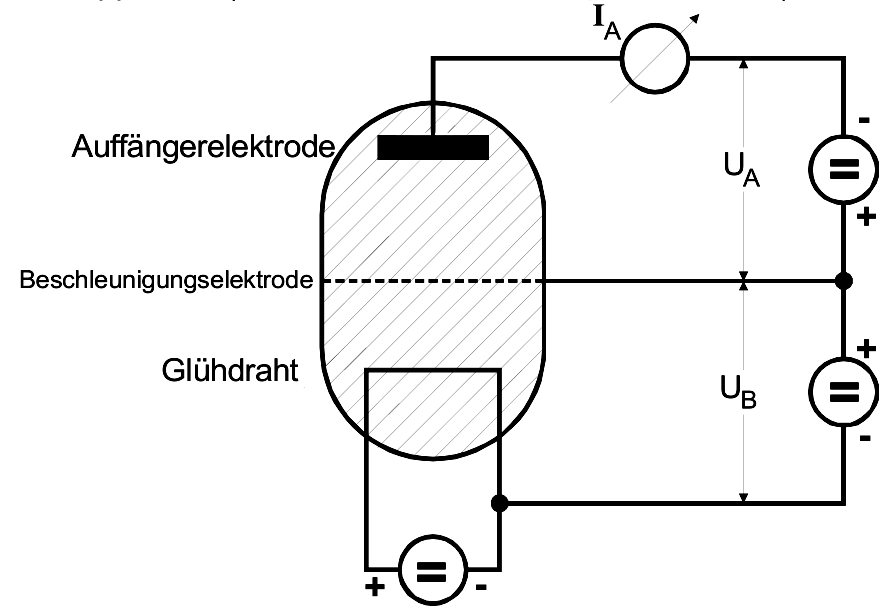
\includegraphics[height=6cm]{ressources/aufbau.png}
  \caption{Systematischer Aufbau einer Franck-Hertz-Röhre. \cite{skript}}
  \label{fig:1}
\end{figure}

Ein Glühdraht, unten in der Abbildung, dient als Elektronenquelle.
Die ausgesandten Elektronen werden durch eine gitterförmige Beschleunigungselektrode in Richtung einer Auffängerelektrode beschleunigt.
An der Beschleunigungselektrode angekommen haben die Elektronen eine kinetische Energie von

\begin{equation}
  \frac{m \cdot v²}{2} = eU_{\text{B}}, \label{eqn:3}
\end{equation}

wenn angenommen wird, dass sie beim Austritt aus dem Glühdraht keine Geschwindigkeit haben.
Nach dem Passieren der Beschleunigungselektrode werden die Elektronen abgebremst, da die Auffängerelektrode negativ geladen wird.
Es sollen nur die Elektronen ankommen die eine Energie von

\begin{equation}
  \frac{m \cdot v²}{2} \ge eU_{\text{A}} \label{eqn:4}
\end{equation}

haben.
Dieses Verfahren wird als Gegenfeldmethode bezeichnet.
Wird nun die Beschleunigungsspannung erhöht, fangen immer mehr Elektronen an, die Auffängerelektrode zu erreichen.
Ab einem bestimmten Energiewert, dargestellt in Gleichung \ref{eqn:1}, der der Anregungsenergie der Hg-Atome entspricht, beginnen sie an Stelle von Elastischen unelastische Stöße mit den Hg-Atomen auszuführen.
Bis zu diesem Phänomen steigt die Stromstärke an der Auffängerelektrode an, ehe sie je absinkt, da die Elektronen nun nicht mehr die nötige Energie besitzen, um sie zu erreichen.
Bei weiterem Erhöhen der Beschleunigungsspannung steigt die Energie der Elektronen nach dem unelastischen Stoß wieder an, bis sie erneut genug Energie für eben diesen haben.
Demnach sollte die Stromstärke der Auffängerelektrode in Abhängigkeit der Beschleunigungsspannung etwa so aussehen wie in Abbildung \ref{fig:2} dargestellt.

\begin{figure}[H]
  \centering
  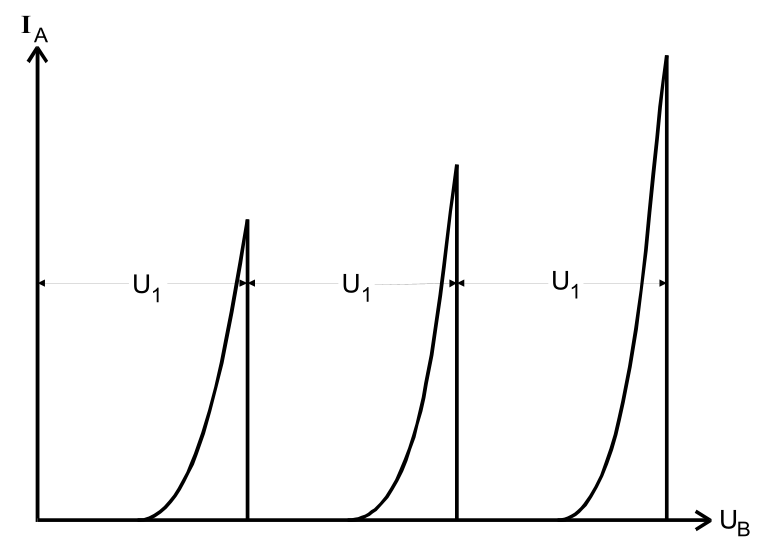
\includegraphics[height=6cm]{ressources/kurve1.png}
  \caption{Theoretische Darstellung einer Franck-Hertz-Kurve. \cite{skript}}
  \label{fig:2}
\end{figure}

Die Stromstärke ist demnach ein Indikator, ab welcher Beschleunigungsspannung die Atome angeregt werden.
Zudem stellt die Differenz $U_1$, zwischen den äquidistanten Maxima,

\begin{equation}
  U_1 = \frac{1}{e}(E_1-E_0), \label{eqn:5}
\end{equation}

multipliziert mit der Elementarladung die Anregungsenergie dar.
Tatsächlich sorgen jedoch Störungseffekte für ein Abrunden und Verbreiterung der Kurve, wobei der Abstand zwischen den Maxima mit zunehmender Spannung $U_{\text{B}}$ leicht zunimmt.

\subsection{Störeffekte}

Ein Störeffekt wird durch das Kontaktpotential ausgelöst.
Das Potential zwischen Elektrode und Heizdraht unterscheidet sich von der angelegten Spannung $U_{\text{B}}$.
Dies passiert, wenn die sich die Austrittsarbeiten der Materialien unterscheiden.
Der Vorteil ist, dass bei hohen Temperaturen dadurch für eine hohe Emissionsrate gesorgt ist.
Nachteilig ist jedoch, dass die angelegte Spannung

\begin{equation}
  U_{\text{B,eff}} = U_{\text{B}} - \frac{1}{e}(\Phi_{\text{B}} - \Phi_{\text{G}}) = U_{\text{B}} - K \label{eqn:6}
\end{equation}

um das Kontaktpotential $K$ verschoben wird.\\
Zudem besitzen die emittierten Elektronen ein Energiespektrum gemäß der Fermi-Dirac-Verteilung.
Sie besitzen beim Austreten also unterschiedliche Energien, was zu einer Verbreiterung der Franck-Hertz-Kurve führt, wodurch sich das Maximum nicht mehr so genau lokalisieren lässt.
Außerdem äußern sich die verschiedenen Energien darin, dass die Stromstärke nicht mehr auf Null, sondern auf ein Stromminimum absinkt.\\
Des Weiteren sorgen die in den Richtungsänderungen resultierenden elastischen Stößen zwischen Auffänger- und Beschleunigungselektrode dafür, dass nicht mehr soviele Elektronen ankommen können.
Es ist ein weiteres Kriterium, welches eine Abflachung und Verbreiterung erklärt.\\
Der letzte große Einfluss wird durch den Hg-Dampfdruck ausgelöst.
Der Dampfdruck bestimmt letztendlich die Wahrscheinlichkeit, mit der es zu einem Stoßprozess kommt.
Damit dies möglichst häufig passiert, aber noch ausreichend viele gemessen werden können, muss die mittlere freie Weglänge $\overline{w}$ der Atome etwa 1000 bis 4000 mal kleiner sein als der Abstand zwischen Kathode und Beschleunigungselektrode.
Für sie gilt

\begin{equation}
  \overline{w} [\text{cm}] = \frac{0,0029}{p_{\text{sätt}}} [\text{p in mbar}] \label{eqn:7},
\end{equation}

wobei

\begin{equation}
  p_{\text{sätt}} = \exp(-6876/T) \label{eqn:8},
\end{equation}

von der Temperatur $T$ abhängt.
Hierbei ist es wichtig ein geeignetes Mittelmaß einzustellen, da bei zu geringem Druck die Elektronen womöglich ohne Stoß die Apparatur durchlaufen und bei zu hohem Druck die Auffängerelektrode nicht erreichen können, da es zu zu starken Richtungsänderungen kommt.








% 2x2 Plot
% \begin{figure*}
%     \centering
%     \begin{subfigure}[b]{0.475\textwidth}
%         \centering
%         \includegraphics[width=\textwidth]{Abbildungen/Schaltung1.pdf}
%         \caption[]%
%         {{\small Schaltung 1.}}
%         \label{fig:Schaltung1}
%     \end{subfigure}
%     \hfill
%     \begin{subfigure}[b]{0.475\textwidth}
%         \centering
%         \includegraphics[width=\textwidth]{Abbildungen/Schaltung2.pdf}
%         \caption[]%
%         {{\small Schaltung 2.}}
%         \label{fig:Schaltung2}
%     \end{subfigure}
%     \vskip\baselineskip
%     \begin{subfigure}[b]{0.475\textwidth}
%         \centering
%         \includegraphics[width=\textwidth]{Abbildungen/Schaltung4.pdf}    % Zahlen vertauscht ... -.-
%         \caption[]%
%         {{\small Schaltung 3.}}
%         \label{fig:Schaltung3}
%     \end{subfigure}
%     \quad
%     \begin{subfigure}[b]{0.475\textwidth}
%         \centering
%         \includegraphics[width=\textwidth]{Abbildungen/Schaltung3.pdf}
%         \caption[]%
%         {{\small Schaltung 4.}}
%         \label{fig:Schaltung4}
%     \end{subfigure}
%     \caption[]
%     {Ersatzschaltbilder der verschiedenen Teilaufgaben.}
%     \label{fig:Schaltungen}
% \end{figure*}
